\section{Yêu cầu chức năng và đặc tả nghiệp vụ}
\label{sec:yeucau_chucnang}
\label{sec:yeucau_chucnang_modules}

Các yêu cầu chức năng được tổ chức theo bốn nhóm nghiệp vụ chính. Use case mô tả mục tiêu và tương tác của người dùng; biểu đồ hoạt động thể hiện các nhánh xử lý chính; biểu đồ tuần tự mô tả sự phối hợp giữa ứng dụng và các hệ thống liên quan.

Các luồng trong chương này mô tả hành vi nghiệp vụ cần hỗ trợ. Mức độ hiện thực và kết quả kiểm thử các luồng nghiệp vụ trên hệ thống tích hợp được trình bày tại Chương~6.

\begin{table}[H]
\centering
\small
\caption{Phạm vi đặc tả theo nhóm nghiệp vụ}
\label{tab:module_owner_scope}
\begin{tabularx}{\textwidth}{|L{4.2cm}|Y|}
\hline
\textbf{Nhóm nghiệp vụ} & \textbf{Phạm vi đặc tả trong chương} \\
\hline
Quản lý hồ sơ cá nhân & Tra cứu các danh mục thông tin lý lịch nhân sự; cập nhật trực tiếp các thông tin được phép hoặc gửi đề xuất kèm minh chứng đối với thông tin cần thẩm định; gửi phản hồi và tra cứu lịch sử xử lý. \\
\hline
Quản lý nghỉ phép & Tra cứu quỹ phép tham khảo, lập và gửi đơn nghỉ phép qua quy trình hướng dẫn, theo dõi và xử lý yêu cầu theo quy trình phê duyệt. \\
\hline
Quản lý công tác & Lập và gửi hồ sơ công tác qua biểu mẫu hướng dẫn 5 bước, kiểm tra xung đột thời gian, theo dõi và xử lý hồ sơ theo quy trình phê duyệt. \\
\hline
Văn phòng số, nhiệm vụ và lịch công tác & Tra cứu, phân công và xử lý văn bản đến; xem văn bản đi, nhiệm vụ và lịch tổng hợp; tạo/đăng ký cuộc họp theo quyền, điểm danh và báo vắng. \\
\hline
\end{tabularx}
\end{table}

\subsection{Quản lý hồ sơ cá nhân}
\label{subsec:req_profile}
\label{subsec:module_profile}

\subsubsection{Mục tiêu và yêu cầu chức năng}

HRM quản lý dữ liệu hồ sơ chính thức; MyHCMUT Mobile cung cấp giao diện native để tra cứu, chỉnh sửa, phản hồi và xem lịch sử. Chính sách do HRM cung cấp xác định cách xử lý từng trường: cập nhật trực tiếp hoặc gửi đề xuất cần thẩm định. Hai loại trường có thể cùng xuất hiện trong một lần thao tác. Mobile dùng chính sách để dựng biểu mẫu; HRM kiểm tra lại quyền, dữ liệu và chính sách khi ghi nhận.

Thông tin được phân thành ba nhóm giao diện trong Bảng~\ref{tab:profile_groups}. Chuyên viên TCNS có quyền thẩm định đối chiếu nội dung đề xuất với dữ liệu hiện tại và minh chứng, sau đó xử lý từng nội dung được phân công.

\begin{table}[H]
\centering
\small
\caption{Phân nhóm danh mục thông tin hồ sơ nhân sự}
\label{tab:profile_groups}
\vspace{0.15cm}
\begin{tabularx}{\textwidth}{|L{4.2cm}|Y|}
\hline
\textbf{Nhóm giao diện} & \textbf{Các danh mục thông tin thành phần} \\
\hline
\textbf{Cá nhân và gia đình} & Thông tin cá nhân cơ bản; Địa chỉ cư trú (thường trú, tạm trú); Quan hệ gia đình (thân nhân, người phụ thuộc). \\
\hline
\textbf{Công tác và đào tạo} & Quá trình công tác / vị trí việc làm hiện tại; Trình độ học vấn, văn bằng chứng chỉ và quá trình đào tạo, bồi dưỡng chuyên môn. \\
\hline
\textbf{Chế độ và thông tin khác} & Quá trình lương và phụ cấp; Khen thưởng; Kỷ luật; Thông tin sức khỏe; Kê khai tài sản / thu nhập. \\
\hline
\end{tabularx}
\end{table}

\begin{table}[H]
\centering
\small
\caption{Yêu cầu chức năng nhóm quản lý hồ sơ cá nhân}
\label{tab:fr_profile}
\begin{tabularx}{\textwidth}{|L{1.8cm}|L{3.5cm}|L{2.5cm}|Y|}
\hline
\textbf{Mã FR} & \textbf{Chức năng} & \textbf{Tác nhân} & \textbf{Mô tả và ràng buộc nghiệp vụ} \\
\hline
FR-PRO-01 & Tra cứu hồ sơ & Nhân sự & Xem các danh mục thông tin lý lịch cá nhân do HRM cung cấp. \\
\hline
FR-PRO-02 & Cập nhật hồ sơ & Nhân sự & Chỉnh sửa bằng biểu mẫu native theo chính sách từng trường; HRM kiểm tra quyền và dữ liệu để cập nhật trực tiếp hoặc tiếp nhận đề xuất kèm minh chứng. \\
\hline
FR-PRO-03 & Thẩm định đề xuất & Chuyên viên TCNS & Đối với đề xuất cần thẩm định, xem xét thông tin sai khác, đối chiếu minh chứng và phê duyệt hoặc từ chối theo thẩm quyền. \\
\hline
FR-PRO-04 & Gửi phản hồi hồ sơ & Nhân sự & Gửi nội dung phản hồi kèm ít nhất một tài liệu minh chứng về danh mục hồ sơ; phản hồi không tự cập nhật dữ liệu chính thức. \\
\hline
FR-PRO-05 & Xem lịch sử hồ sơ & Nhân sự & Quan sát yêu cầu và nhật ký cập nhật; đối chiếu dữ liệu ban đầu với dữ liệu mới hoặc đề xuất theo từng trường, kèm trạng thái xử lý do HRM trả về. \\
\hline

\end{tabularx}
\end{table}

\subsubsection{Đặc tả Use Case}

UC-PRO-01 đến UC-PRO-05 lần lượt tương ứng FR-PRO-01 đến FR-PRO-05. Hình~\ref{fig:uc_profile} minh họa các nhánh nghiệp vụ; UC-PRO-05 bổ sung chức năng lịch sử.

\begin{figure}[H]
\centering
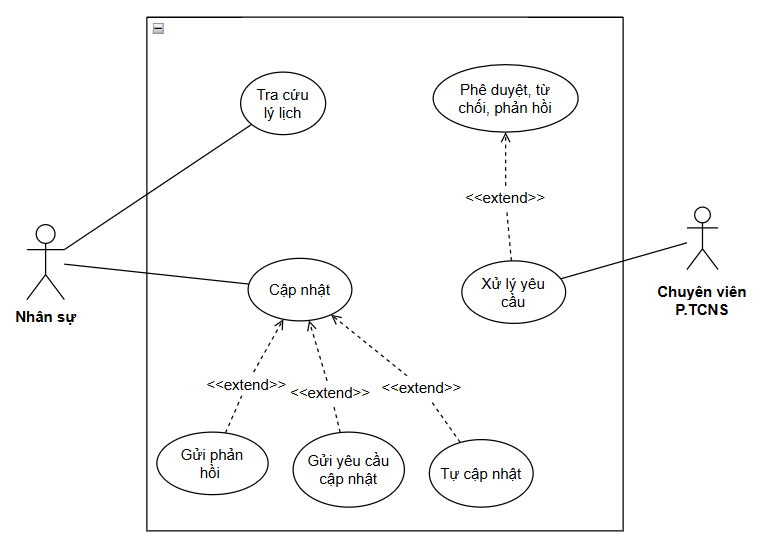
\includegraphics[width=\linewidth]{image/usecase/UC_PROFILE.png}
\caption{Sơ đồ Đặc tả Use case nhóm Quản lý hồ sơ cá nhân}
\label{fig:uc_profile}
\end{figure}

\usecasespec{
  id={UC-PRO-01},
  name={Tra cứu hồ sơ nhân sự},
  shortname={Tra cứu hồ sơ},
  actor={Nhân sự},
  desc={Cho phép nhân sự tra cứu các danh mục thông tin lý lịch cá nhân được cung cấp bởi hệ thống HRM.},
  pre={Nhân sự đã đăng nhập thành công vào ứng dụng MyHCMUT Mobile.},
  trigger={Người dùng chọn mục ``Hồ sơ cá nhân'' trên ứng dụng di động.},
  mainflow={
    1. Người dùng mở giao diện hồ sơ cá nhân trên ứng dụng. \newline
    2. Ứng dụng hiển thị thông tin tổng quan và ba nhóm giao diện chính. \newline
    3. Người dùng lựa chọn nhóm và danh mục thông tin cần xem. \newline
    4. Ứng dụng tải và hiển thị chi tiết các trường dữ liệu tương ứng từ hệ thống HRM.
  },
  altflow={
    - \textit{Luồng 2a (Làm mới dữ liệu):} Người dùng thực hiện làm mới để yêu cầu ứng dụng tải dữ liệu mới nhất từ hệ thống HRM.
  },
  exflow={
    - \textit{Ngoại lệ 4a (Lỗi kết nối):} Khi không thể tải dữ liệu từ hệ thống HRM, ứng dụng sử dụng dữ liệu hồ sơ đã lưu tạm trước đó nếu có và thông báo trạng thái kết nối cho người dùng. Nếu chưa có dữ liệu lưu tạm, ứng dụng thông báo không thể tải dữ liệu.
  },
  post={Người dùng xem được dữ liệu hồ sơ mới nhất tải được từ HRM hoặc dữ liệu đã lưu tạm gần nhất khi không thể kết nối.},
  label={tab:uc_pro_01}
}

\usecasespec{
  id={UC-PRO-02},
  name={Cập nhật hồ sơ cá nhân},
  shortname={Cập nhật hồ sơ},
  actor={Nhân sự},
  desc={Cho phép nhân sự cập nhật thông tin hồ sơ theo phạm vi quyền; HRM ghi nhận trực tiếp các thông tin được phép và tiếp nhận đề xuất đối với thông tin cần thẩm định.},
  pre={Nhân sự đã đăng nhập vào MyHCMUT Mobile và đang xem hồ sơ của bản thân.},
  trigger={Người dùng chọn chức năng cập nhật tại danh mục thông tin tương ứng.},
  mainflow={
    1. Người dùng chọn cập nhật thông tin hồ sơ. \newline
    2. Ứng dụng tải dữ liệu hiện tại và chính sách cập nhật từ HRM, sau đó mở biểu mẫu Flutter của danh mục được hỗ trợ. \newline
    3. Người dùng điều chỉnh các thông tin cần thay đổi và cung cấp tài liệu minh chứng đối với những nội dung yêu cầu minh chứng. \newline
    4. Ứng dụng kiểm tra dữ liệu đầu vào và minh chứng theo chính sách, chỉ gửi những trường thực sự thay đổi khi người dùng xác nhận. \newline
    5. HRM kiểm tra quyền, tính hợp lệ của dữ liệu và chính sách áp dụng cho từng trường thông tin. \newline
    6. Các trường được phép tự cập nhật được ghi nhận trực tiếp; các trường cần thẩm định được ghi nhận thành nội dung đề xuất chờ xử lý. \newline
    7. Hệ thống phản hồi kết quả để người dùng theo dõi thông tin hoặc trạng thái đề xuất tương ứng.
  },
  exflow={
    - \textit{Ngoại lệ 4a (Thiếu tài liệu minh chứng):} Khi thiếu tài liệu minh chứng đối với nội dung yêu cầu minh chứng, hệ thống thông báo để người dùng bổ sung trước khi tiếp nhận nội dung tương ứng. \newline
    - \textit{Ngoại lệ 4b (Mất kết nối):} Ứng dụng thông báo lỗi; không coi dữ liệu đang nhập là thay đổi đã được HRM lưu. Khi chưa xác định kết quả gửi, người dùng cần kiểm tra hồ sơ hoặc lịch sử trước khi gửi lại. \newline
    - \textit{Ngoại lệ 5a (Không đáp ứng điều kiện nghiệp vụ):} Khi tồn tại điều kiện nghiệp vụ không cho phép tiếp nhận thay đổi, hệ thống từ chối thao tác và phản hồi nguyên nhân cho người dùng.
  },
  post={Thông tin được phép đã được cập nhật vào hồ sơ; các thông tin cần thẩm định được ghi nhận thành đề xuất chờ xử lý.},
  label={tab:uc_pro_02}
}

\usecasespec{
  id={UC-PRO-03},
  name={Thẩm định thay đổi hồ sơ},
  shortname={Thẩm định thay đổi hồ sơ},
  actor={Chuyên viên Phòng Tổ chức Nhân sự có thẩm quyền},
  desc={Cho phép chuyên viên TCNS có thẩm quyền đối chiếu nội dung đề xuất với dữ liệu hiện tại và tài liệu minh chứng, sau đó xử lý các nội dung thay đổi theo phạm vi được phân công.},
  pre={Chuyên viên đã đăng nhập và tài khoản được phân quyền thẩm định hồ sơ nhân sự.},
  trigger={Chuyên viên mở danh sách các đề xuất cập nhật hồ sơ đang chờ xử lý.},
  mainflow={
    1. Chuyên viên mở danh sách đề xuất cập nhật hồ sơ chờ xử lý. \newline
    2. Chọn một đề xuất cụ thể để xem chi tiết. \newline
    3. Ứng dụng hiển thị thông tin hiện tại và nội dung đề xuất để chuyên viên đối chiếu, kèm tài liệu minh chứng tương ứng. \newline
    4. Chuyên viên lựa chọn phê duyệt hoặc từ chối đối với từng nội dung thay đổi theo phạm vi được cấp quyền. \newline
    5. Đối với thao tác từ chối, ứng dụng yêu cầu chuyên viên nhập lý do. \newline
    6. Hệ thống ghi nhận kết quả xử lý của từng nội dung. Khi toàn bộ nội dung thuộc đề xuất đã được xử lý, trạng thái của đề xuất được cập nhật tương ứng và các thay đổi được chấp thuận được phản ánh vào hồ sơ. \newline
    7. Kết quả xử lý được ghi nhận để người đề xuất theo dõi.
  },
  altflow={
    - \textit{Luồng 4a (Xử lý từng phần):} Một đề xuất có thể được xử lý từng phần; các nội dung đã được xử lý được ghi nhận kết quả trong khi các nội dung còn lại tiếp tục chờ xử lý.
  },
  exflow={
    - \textit{Ngoại lệ 4a (Trạng thái hoặc quyền xử lý thay đổi):} Khi thao tác không còn hợp lệ do trạng thái đề xuất đã thay đổi hoặc người dùng không còn quyền xử lý nội dung tương ứng, hệ thống từ chối thao tác và yêu cầu làm mới trạng thái hiện tại.
  },
  post={Kết quả xử lý của từng nội dung được ghi nhận; khi toàn bộ nội dung đã được xử lý, đề xuất đạt trạng thái kết thúc tương ứng và dữ liệu hồ sơ phản ánh các thay đổi đã được chấp thuận.},
  label={tab:uc_pro_03}
}

\usecasespec{
 id={UC-PRO-04}, name={Gửi phản hồi hồ sơ}, shortname={Gửi phản hồi}, actor={Nhân sự},
 desc={Ghi nhận phản hồi liên quan đến một danh mục hồ sơ bằng giao diện native.},
 pre={Người dùng đã đăng nhập và có quyền gửi phản hồi tại danh mục tương ứng.},
 trigger={Người dùng chọn gửi phản hồi trong menu thao tác hồ sơ.},
 mainflow={1. Ứng dụng mở biểu mẫu phản hồi của danh mục được chọn. \newline
 2. Người dùng nhập nội dung phản hồi và đính kèm ít nhất một tài liệu minh chứng. \newline
 3. Ứng dụng gửi nội dung theo hợp đồng API phản hồi của HRM. \newline
 4. HRM kiểm tra quyền và dữ liệu, ghi nhận phản hồi rồi trả kết quả. \newline
 5. Ứng dụng thông báo kết quả; người dùng theo dõi tại lịch sử hồ sơ.},
 exflow={- Thiếu nội dung hoặc minh chứng: yêu cầu bổ sung trước khi gửi. \newline
 - Dữ liệu không hợp lệ, quyền thay đổi hoặc lỗi kết nối: hiển thị lỗi; không thông báo gửi thành công khi backend chưa xác nhận.},
 post={Phản hồi hợp lệ được ghi nhận; dữ liệu hồ sơ chính thức không tự thay đổi chỉ vì đã gửi phản hồi.}, label={tab:uc_pro_04}
}
\usecasespec{
 id={UC-PRO-05}, name={Xem lịch sử hồ sơ}, shortname={Xem lịch sử}, actor={Nhân sự},
 desc={Tra cứu các yêu cầu, nội dung thay đổi và nhật ký mà HRM cho phép người dùng xem.},
 pre={Người dùng đã đăng nhập và được truy cập lịch sử hồ sơ tương ứng.},
 trigger={Người dùng chọn mục lịch sử hồ sơ.},
 mainflow={1. Ứng dụng yêu cầu lịch sử từ HRM. \newline
 2. HRM xác định phạm vi dữ liệu theo phiên và quyền, trả yêu cầu cùng nhật ký liên quan. \newline
 3. Ứng dụng trình bày hai nhóm yêu cầu và thay đổi đã ghi nhận, kèm thời điểm, trạng thái và thông tin xử lý được backend trả về. \newline
 4. Người dùng mở chi tiết để quan sát các trường khác nhau, đối chiếu dữ liệu ban đầu với dữ liệu mới hoặc nội dung đề xuất; xem lý do và minh chứng nếu có.},
 altflow={- Không có lịch sử: ứng dụng hiển thị trạng thái danh sách rỗng.},
 exflow={- Không thể tải hoặc không đủ quyền: thông báo lỗi, không diễn giải dữ liệu chưa tải là không có yêu cầu.},
 post={Người dùng xem được lịch sử do HRM cung cấp; thao tác này không thay đổi trạng thái yêu cầu.}, label={tab:uc_pro_05}
}

UC-PRO-05 sử dụng giá trị trước/sau do HRM trả về để đối chiếu từng trường có dữ liệu lịch sử; nội dung chờ duyệt hoặc bị từ chối chưa phải dữ liệu có hiệu lực. Phạm vi chỉnh sửa native gồm thông tin cá nhân, địa chỉ, ngân hàng/bảo hiểm, gia đình, công tác ngoài Trường, đào tạo và kê khai tài sản/thu nhập. Chính sách chỉnh sửa và minh chứng được áp dụng riêng theo danh mục, không mặc định mọi trường đều được sửa hoặc đều cần tệp.

\subsubsection{Biểu đồ hoạt động}

Hình~\ref{fig:act_profile_request} thể hiện cập nhật trực tiếp và thẩm định đề xuất theo từng nhóm trường; cả hai hướng có thể cùng xuất hiện trong một lần cập nhật.

\begin{figure}[H]
\centering
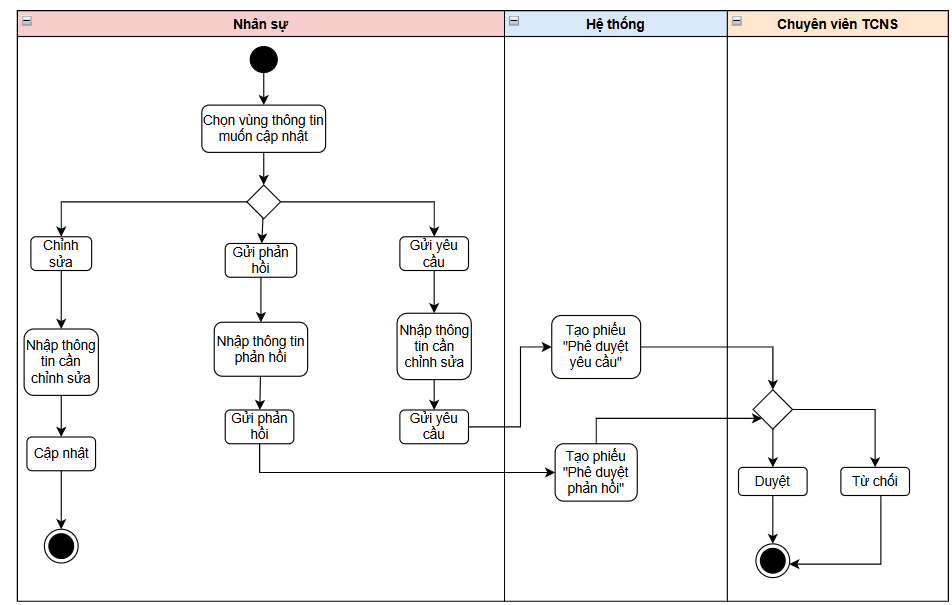
\includegraphics[width=\linewidth]{image/uml/profile_activity.png}
\caption{Biểu đồ hoạt động Quy trình cập nhật hồ sơ cá nhân}
\label{fig:act_profile_request}
\end{figure}

\subsubsection{Biểu đồ tuần tự}

Hình~\ref{fig:seq_profile_request} minh họa lấy dữ liệu/chính sách, gửi nội dung thay đổi và xử lý tại HRM. Hai nhánh cập nhật trực tiếp và đề xuất áp dụng theo trường. Hợp đồng API và truyền tệp được trình bày tại Chương~5.

\begin{figure}[H]
\centering
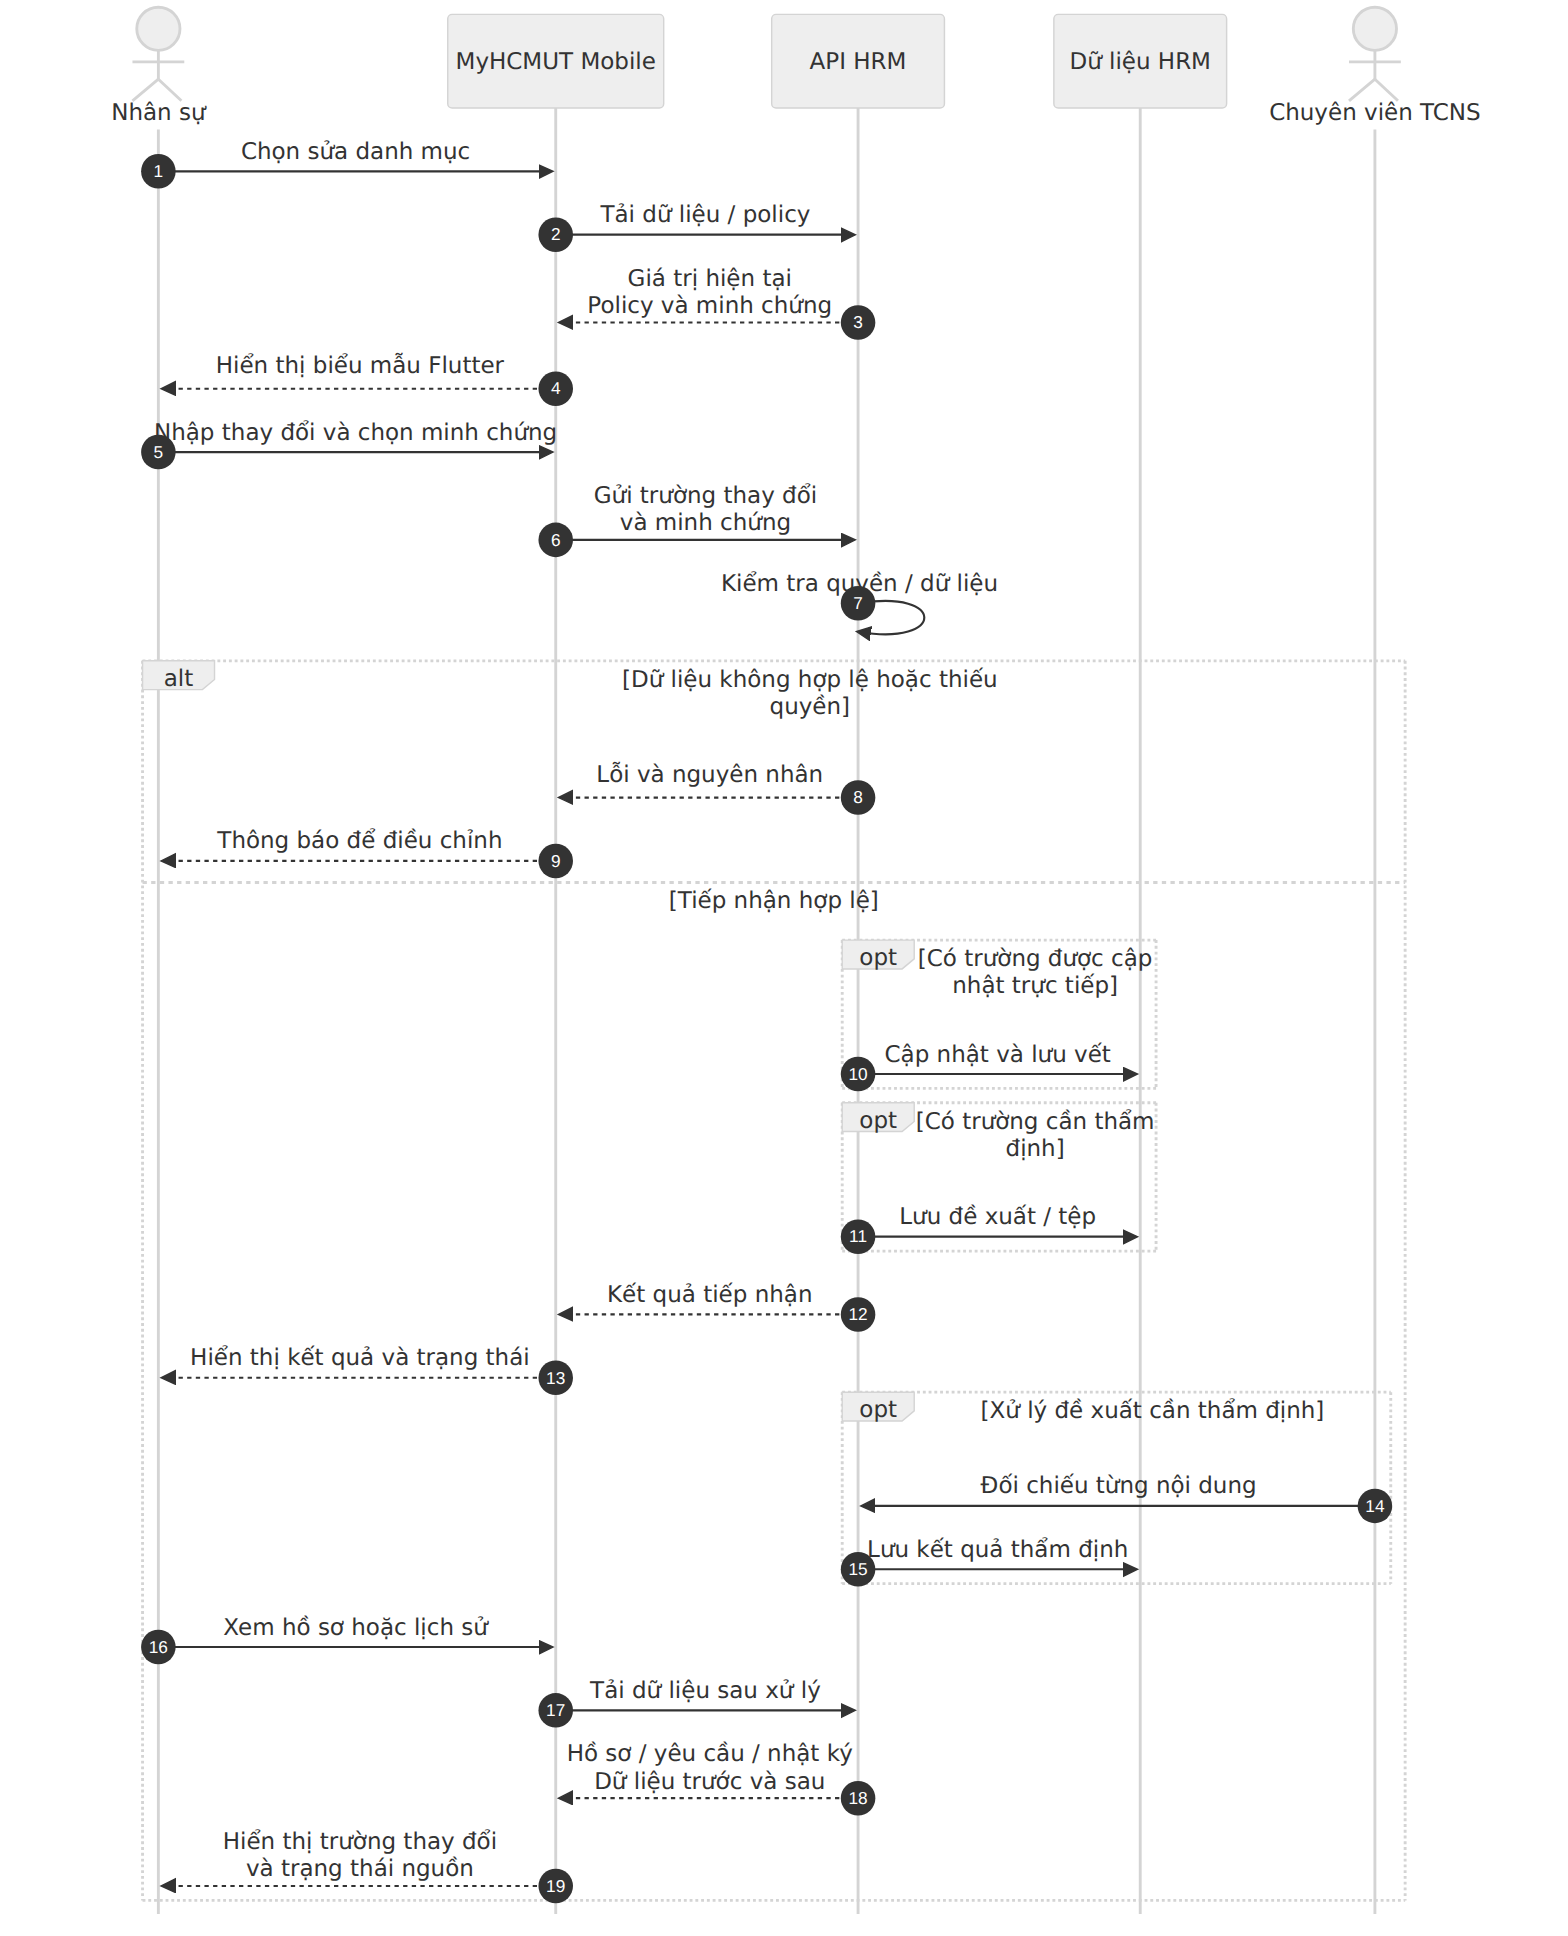
\includegraphics[width=\linewidth]{image/uml/seq_profile_request.png}
\caption{Biểu đồ tuần tự Cập nhật hồ sơ cá nhân}
\label{fig:seq_profile_request}
\end{figure}

\subsection{Quản lý nghỉ phép}
\label{subsec:req_leave}
\label{subsec:module_leave}

\subsubsection{Mục tiêu và yêu cầu chức năng}

Ứng dụng hỗ trợ tra cứu quỹ phép tham khảo, lập đơn theo biểu mẫu ba bước, theo dõi và xử lý theo thẩm quyền. Kiểm tra ngày, số dư và xung đột trên mobile hỗ trợ hoàn thiện dữ liệu; backend HRM thực hiện kiểm tra nghiệp vụ cuối cùng và xử lý việc chuyển trạng thái hồ sơ.

\begin{table}[H]
\centering
\small
\caption{Yêu cầu chức năng nhóm quản lý nghỉ phép}
\label{tab:fr_leave}
\begin{tabularx}{\textwidth}{|L{1.8cm}|L{3.5cm}|L{2.5cm}|Y|}
\hline
\textbf{Mã FR} & \textbf{Chức năng} & \textbf{Tác nhân} & \textbf{Mô tả và ràng buộc nghiệp vụ} \\
\hline
FR-LEV-01 & Tra cứu quỹ phép và đơn & Nhân sự & Xem số dư quỹ phép năm tham khảo, lọc danh sách đơn theo năm và trạng thái xử lý. \\
\hline
FR-LEV-02 & Lập và gửi đơn nghỉ phép & Nhân sự & Nhập liệu theo biểu mẫu 3 bước, đính kèm minh chứng, lưu nháp hoặc gửi duyệt khi đáp ứng điều kiện nghiệp vụ. \\
\hline
FR-LEV-03 & Quản lý đơn đã tạo & Nhân sự & Chỉnh sửa hoặc xóa đơn ở trạng thái Nháp; chỉnh sửa và gửi lại đơn Bị trả lại. Đơn đã gửi không mặc định có thao tác thu hồi cho người lập. \\
\hline
FR-LEV-04 & Phê duyệt theo thẩm quyền & Cấp phê duyệt & Xem xét nội dung, minh chứng và phê duyệt, từ chối hoặc trả lại đơn theo thẩm quyền được phân công. \\
\hline
\end{tabularx}
\end{table}

Trong quy trình hiện thực, thao tác lưu giữ đơn ở trạng thái Nháp, còn thao tác gửi mới chuyển đơn sang bước chờ duyệt. Quyền thu hồi của người có thẩm quyền thuộc luồng xử lý riêng, không đồng nhất với quyền xóa đơn Nháp của người lập.

\subsubsection{Đặc tả Use Case}

UC-LEV-01 cụ thể hóa FR-LEV-01 và FR-LEV-03; UC-LEV-02 gắn với FR-LEV-02, còn UC-LEV-03 gắn với FR-LEV-04. Hình~\ref{fig:uc_leave} thể hiện các nhóm thao tác tương ứng.

\begin{figure}[H]
\centering
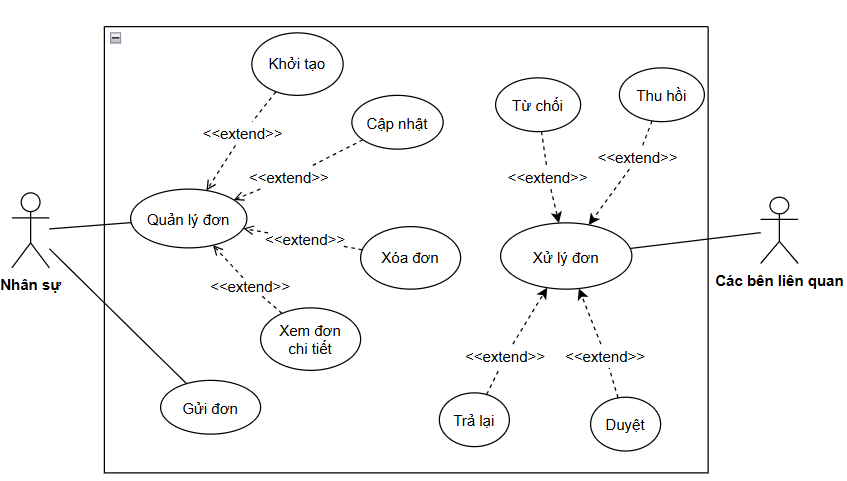
\includegraphics[width=\linewidth]{image/usecase/UC_LEAVE.png}
\caption{Sơ đồ Đặc tả Use case nhóm Quản lý nghỉ phép}
\label{fig:uc_leave}
\end{figure}

\usecasespec{
  id={UC-LEV-01},
  name={Quản lý đơn nghỉ phép cá nhân},
  shortname={Quản lý đơn cá nhân},
  actor={Nhân sự},
  desc={Cho phép nhân sự theo dõi số dư quỹ phép năm, tra cứu danh sách đơn và tiến trình duyệt; chỉnh sửa hoặc xóa đơn Nháp, chỉnh sửa và gửi lại đơn Bị trả lại.},
  pre={Nhân sự đã đăng nhập thành công vào ứng dụng MyHCMUT Mobile.},
  trigger={Người dùng chọn chức năng ``Nghỉ phép'' trên màn hình chính.},
  mainflow={
    1. Người dùng mở mục ``Nghỉ phép'' để xem số dư quỹ phép tham khảo và danh sách đơn đã lập. \newline
    2. Người dùng lọc danh sách hoặc chọn một đơn để xem trạng thái và tiến trình xử lý. \newline
    3. Với đơn Nháp, người dùng có thể tiếp tục chỉnh sửa hoặc xóa đơn. \newline
    4. HRM kiểm tra người lập và trạng thái đơn trước khi ghi nhận thao tác hợp lệ.
  },
  altflow={
    - \textit{Luồng 3a (Sửa đơn bị trả lại):} Với đơn ở trạng thái Bị trả lại, người dùng chọn chỉnh sửa để bổ sung thông tin và gửi lại. \newline
    - \textit{Luồng 3b (Theo dõi đơn đã gửi):} Với đơn đang chờ duyệt, người dùng xem trạng thái và lịch sử xử lý; ứng dụng không mặc định cung cấp thao tác thu hồi cho người lập.
  },
  exflow={
    - \textit{Ngoại lệ 4a (Trạng thái đã thay đổi):} Nếu đơn không còn ở trạng thái cho phép chỉnh sửa hoặc xóa, HRM từ chối thao tác và ứng dụng cập nhật trạng thái mới.
  },
  post={Nhân sự nắm bắt thông tin quỹ phép và trạng thái các đơn; những thay đổi hợp lệ đối với đơn Nháp hoặc đơn Bị trả lại được ghi nhận trên HRM.},
  label={tab:uc_lev_01}
}

\usecasespec{
  id={UC-LEV-02},
  name={Lập và gửi đơn nghỉ phép},
  shortname={Lập và gửi đơn nghỉ phép},
  actor={Nhân sự},
  desc={Cho phép nhân sự lập mới đơn nghỉ phép qua quy trình hướng dẫn 3 bước, kiểm tra thời gian và số dư phép, đính kèm minh chứng và gửi duyệt.},
  pre={Nhân sự đã đăng nhập vào hệ thống và có quyền lập đơn nghỉ phép.},
  trigger={Người dùng nhấn nút tạo mới đơn nghỉ phép trên giao diện ứng dụng.},
  mainflow={
    1. Người dùng chọn tạo mới đơn nghỉ phép; ứng dụng kiểm tra ngày đăng ký có hợp lệ trước khi yêu cầu tạo nháp. \newline
    2. Khi ngày đăng ký hợp lệ, hệ thống khởi tạo bản ghi nháp. \newline
    3. Người dùng nhập thông tin nghỉ phép và đính kèm minh chứng khi được yêu cầu. \newline
    4. Người dùng rà soát thông tin và gửi đơn. \newline
    5. HRM kiểm tra các điều kiện nghiệp vụ và tiếp nhận đơn hợp lệ vào quy trình chờ duyệt.
  },
  altflow={
    - \textit{Luồng 3a (Lưu nháp):} Người dùng chọn lưu nháp tại bất kỳ bước nào để tiếp tục hoàn thiện sau. \newline
    - \textit{Luồng 3b (Thoát biểu mẫu):} Người dùng xác nhận thoát; dữ liệu chưa lưu trên ứng dụng bị bỏ. Bản ghi nháp đã tạo trên HRM vẫn tồn tại, có thể mở lại hoặc xóa bằng thao tác riêng.
  },
  exflow={
    - \textit{Ngoại lệ 1a (Ngày đăng ký không hợp lệ):} Ứng dụng thông báo nguyên nhân và không tạo bản ghi nháp. \newline
    - \textit{Ngoại lệ 3a (Xung đột lịch trình):} Khoảng thời gian nghỉ trùng lặp với kế hoạch công tác hoặc đơn khác $\rightarrow$ hệ thống cảnh báo và yêu cầu điều chỉnh. \newline
    - \textit{Ngoại lệ 3b (Vượt số dư quỹ phép):} Số ngày đăng ký vượt quá số dư phép năm còn lại $\rightarrow$ hệ thống cảnh báo để người dùng điều chỉnh. \newline
    - \textit{Ngoại lệ 3c (Quá hạn đăng ký):} Khi kiểm tra thời hạn xác định không thể tạo đơn nghỉ phép thông thường, ứng dụng thông báo nguyên nhân và điều hướng người dùng đến điểm truy cập phân hệ Giải trình. Việc lập và xử lý Giải trình không thuộc phạm vi hiện thực của use case này.
  },
  post={Khi gửi thành công, đơn được ghi nhận ở bước chờ duyệt và phát sinh thông báo theo quy trình. Nếu chỉ lưu hoặc thoát sau khi tạo nháp, đơn vẫn ở trạng thái Nháp.},
  label={tab:uc_lev_02}
}

\usecasespec{
  id={UC-LEV-03},
  name={Xử lý đơn nghỉ phép},
  shortname={Xử lý đơn nghỉ phép},
  actor={Lãnh đạo Đơn vị, Chuyên viên Phòng Tổ chức Nhân sự, Ban Giám hiệu},
  desc={Cho phép người có thẩm quyền thẩm định nội dung đơn, kiểm tra tài liệu minh chứng và thực hiện phê duyệt, từ chối hoặc yêu cầu bổ sung thông tin.},
  pre={Người duyệt đã đăng nhập và đơn đang ở bước thuộc thẩm quyền xử lý của tài khoản.},
  trigger={Người duyệt mở danh sách đơn chờ xử lý từ ứng dụng hoặc qua thông báo nhắc việc.},
  mainflow={
    1. Người duyệt mở danh sách đơn nghỉ phép chờ xử lý thuộc thẩm quyền phân công. \newline
    2. Chọn xem chi tiết một đơn để kiểm tra nội dung và minh chứng liên quan. \newline
    3. Người duyệt lựa chọn hành động: \textit{Phê duyệt}, \textit{Từ chối} hoặc \textit{Trả lại}. \newline
    4. HRM kiểm tra quyền và trạng thái đơn hiện tại, rồi ghi nhận kết quả xử lý hoặc chuyển đơn sang bước tiếp theo. \newline
    5. Hệ thống thông báo kết quả cho nhân sự lập đơn; số dư phép được cập nhật khi đơn hoàn tất theo quy tắc nghiệp vụ.
  },
  altflow={
    - \textit{Luồng 3a (Xử lý đồng loạt):} Người duyệt chọn nhiều đơn hợp lệ trên danh sách và thực hiện phê duyệt hàng loạt. \newline
    - \textit{Luồng 3b (Trả lại yêu cầu chỉnh sửa):} Người duyệt chọn ``Trả lại'' kèm ý kiến yêu cầu $\rightarrow$ đơn chuyển sang trạng thái Bị trả lại để nhân sự hoàn thiện.
  },
  exflow={
    - \textit{Ngoại lệ 3a (Từ chối đơn):} Người duyệt bắt buộc nhập lý do từ chối trước khi hệ thống ghi nhận kết quả. \newline
    - \textit{Ngoại lệ 4a (Trạng thái không phù hợp):} Khi HRM xác định đơn không còn ở bước cho phép xử lý, thao tác bị từ chối và người dùng cần tải lại dữ liệu. Kiểm tra này không được xem là bảo đảm chống mọi thao tác phê duyệt đồng thời.
  },
  post={Đơn được chuyển sang bước tiếp theo, trả lại hoặc kết thúc theo quyết định được HRM ghi nhận; dữ liệu nghỉ phép được cập nhật khi duyệt bước cuối theo quy trình.},
  label={tab:uc_lev_03}
}

\subsubsection{Biểu đồ hoạt động}

Hình~\ref{fig:act_leave_submit} mô tả lập đơn và luân chuyển phê duyệt. Khi quá hạn, ứng dụng thông báo và điều hướng đến điểm truy cập Giải trình; quy trình Giải trình nằm ngoài phạm vi use case nghỉ phép hiện tại.

\begin{figure}[H]
\centering
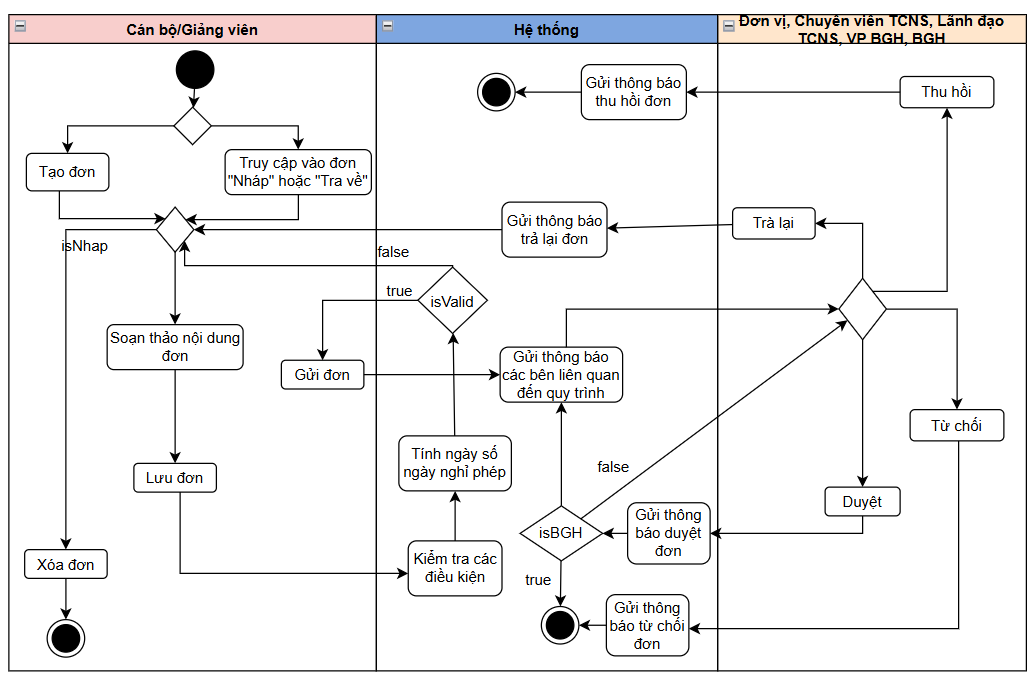
\includegraphics[width=\linewidth]{image/uml/leave_activity.png}
\caption{Biểu đồ hoạt động Quy trình nghỉ phép}
\label{fig:act_leave_submit}
\end{figure}

\subsubsection{Biểu đồ tuần tự}
Hình~\ref{fig:seq_leave_submit} minh họa UC-LEV-02: khởi tạo nháp, hoàn thiện dữ liệu và gửi vào quy trình chờ duyệt.

\begin{figure}[H]
\centering
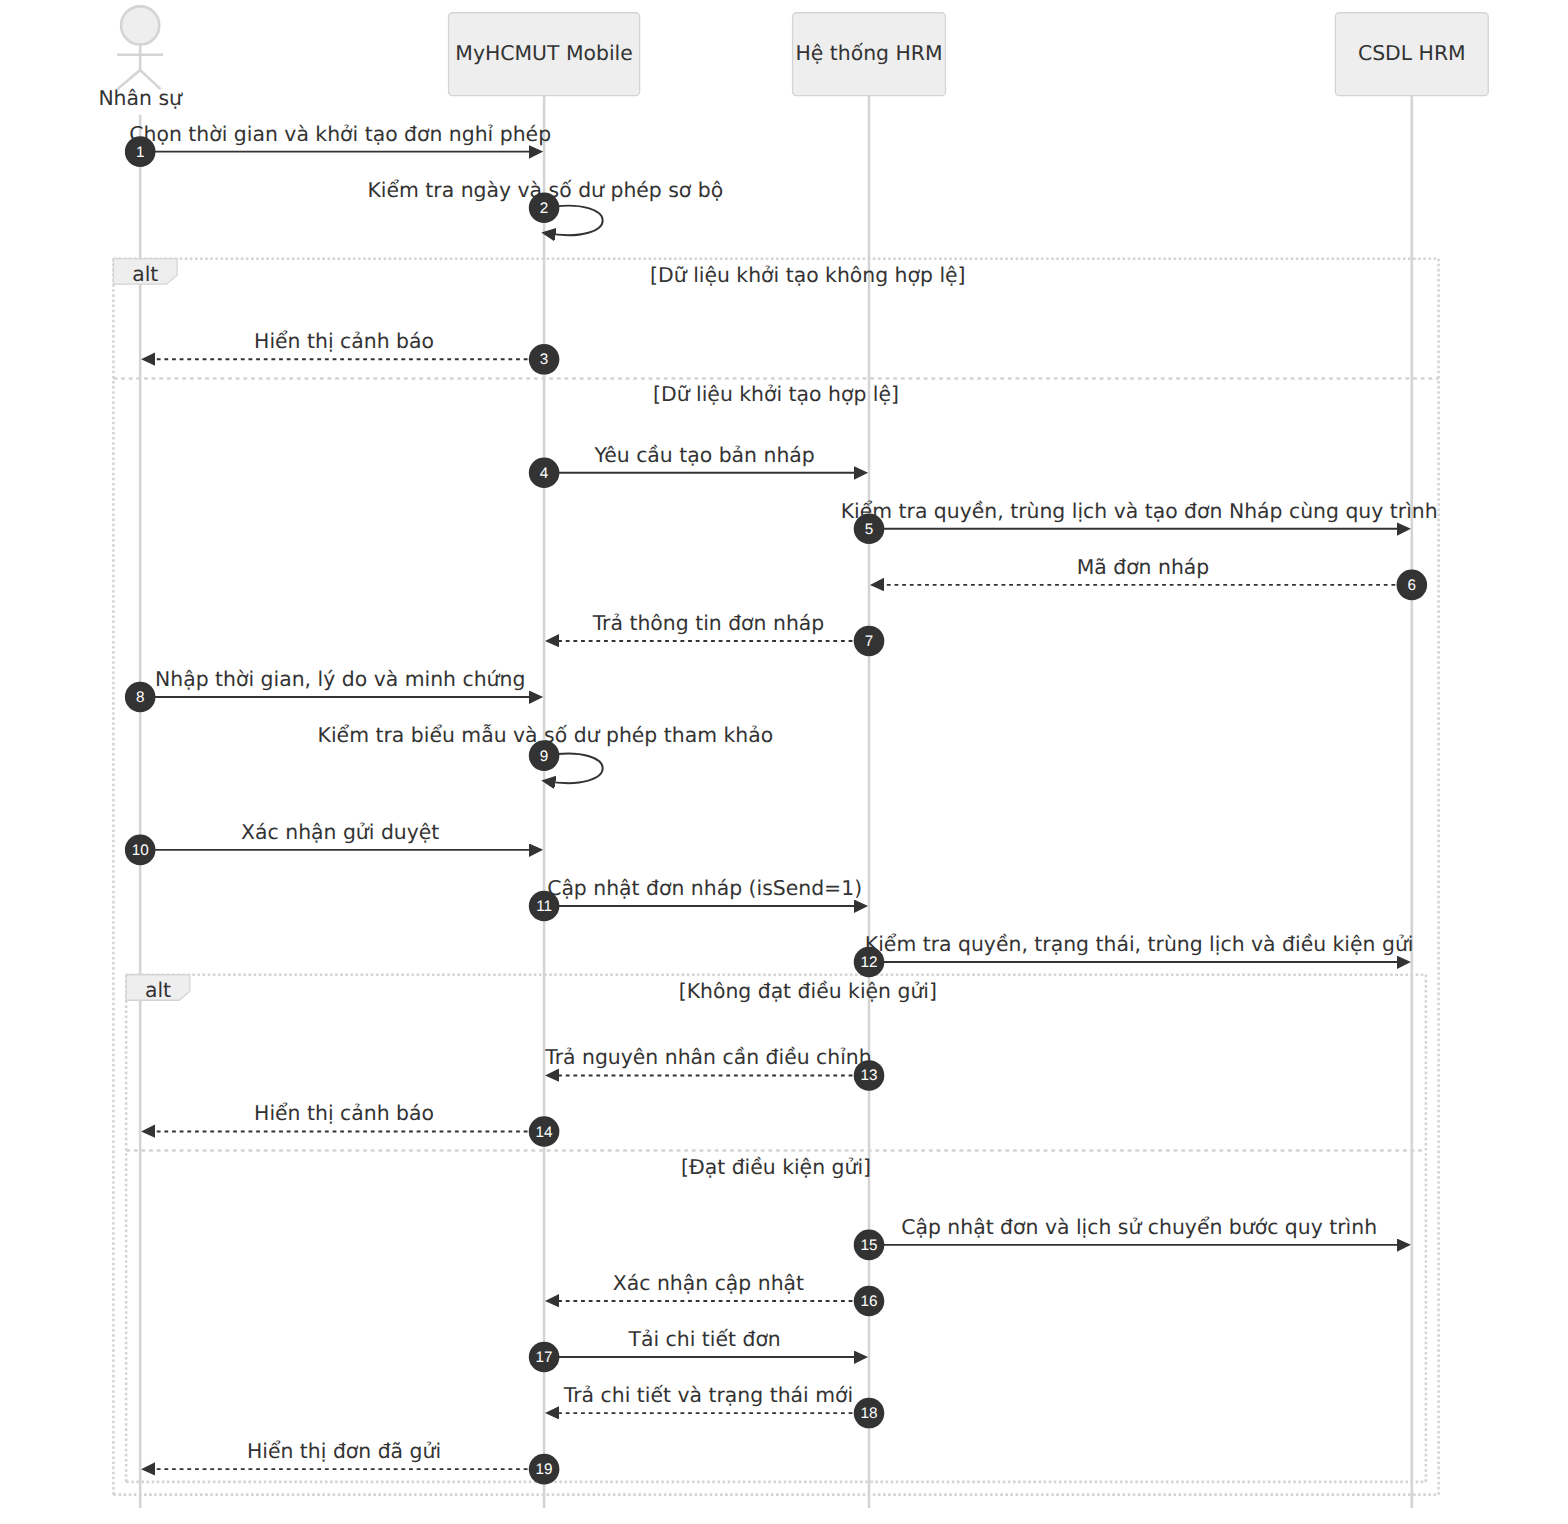
\includegraphics[width=\linewidth]{image/uml/seq_leave_submit.png}
\caption{Biểu đồ tuần tự Gửi yêu cầu nghỉ phép}
\label{fig:seq_leave_submit}
\end{figure}

\subsection{Phân hệ quản lý công tác}
\label{subsec:business_trip}

\subsubsection{Mục tiêu}
Công tác là một trong những nghiệp vụ quan trọng hỗ trợ người lao động toàn trường tối
ưu quá trình quản lý thông tin quy trình các chuyến đi công tác. Quy trình quản lý thông tin công tác bắt đầu từ việc
đăng ký công tác của cán bộ. Đơn đăng ký công tác sẽ được gửi đến các bên liên quan để thẩm định và phê duyệt, người dùng cũng nắm bắt được thông tin về tiến độ các bước phê duyệt.
Sau khi được phê duyệt, cán bộ sẽ thực hiện chuyến công tác và báo cáo kết quả (nếu có).


\subsubsection{Yêu cầu chức năng}

\begin{table}[H]
\centering
\small
\caption{Yêu cầu chức năng nhóm quản lý công tác}
\label{tab:fr_business_trip}
\begin{tabularx}{\textwidth}{|L{1.8cm}|L{3.5cm}|L{2.5cm}|Y|}
\hline
\textbf{Mã FR} & \textbf{Chức năng} & \textbf{Tác nhân} & \textbf{Mô tả và ràng buộc nghiệp vụ} \\
\hline
FR-BTR-01 & Tra cứu đơn & Cán bộ, Giảng viên & Xem danh sách đơn công tác cá nhân, lọc theo trạng thái và xem chi tiết tiến trình duyệt. \\
\hline
FR-BTR-02 & Tạo và gửi đơn & Cán bộ, Giảng viên & Tạo phiếu đăng ký công tác, điền thông tin và gửi cho các bên liên quan phê duyệt. \\
\hline
FR-BTR-03 & Quản lý nháp và điều chỉnh & Cán bộ, Giảng viên & Chỉnh sửa hoặc xóa phiếu Nháp; chỉnh sửa và gửi lại phiếu Bị trả lại. Người lập không tự thu hồi phiếu đã gửi. \\
\hline
FR-BTR-04 & Xử lý đơn & Các bên liên quan & Xem xét thông tin đơn đăng ký, minh chứng và thực hiện các thao tác như: phê duyệt, từ chối hoặc trả lại đơn theo thẩm quyền. \\
\hline
FR-BTR-05 & Thu hồi đơn & Chuyên viên P.TCNS/BGH & Thu hồi đơn đăng ký công tác ở bất kỳ bước nào trong quy trình. \\
\hline
\end{tabularx}
\end{table}

\subsubsection{Đặc tả Use Case}
\begin{figure}[H]
    \centering
    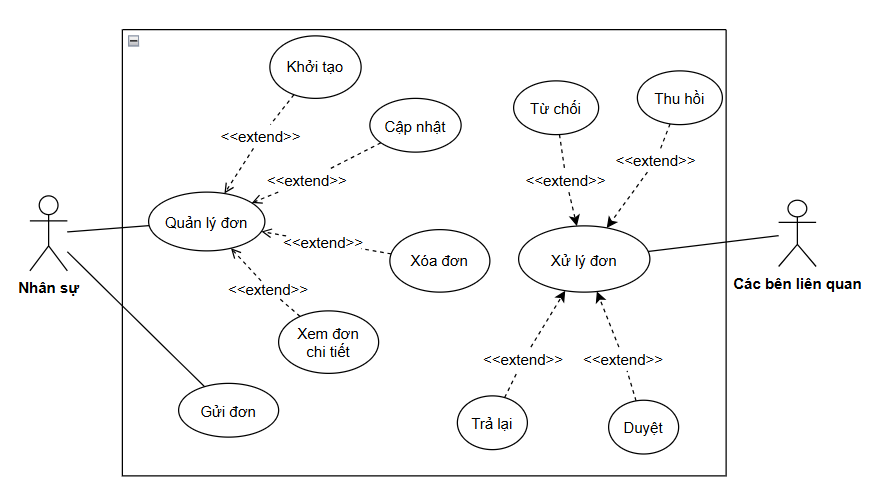
\includegraphics[width=\linewidth]{image/usecase/UC_BT.png}
    \caption{\textit{Sơ đồ use-case quản lý công tác}}
    \label{fig:BT_UC}
\end{figure}

\usecasespec{
    id={UC-BT-01},
    name={Soạn thảo đơn đăng ký công tác},
    actor={Cán bộ / Giảng viên},
    pre={Đã đăng nhập vào ứng dụng và tài khoản có quyền tạo đơn đăng ký công tác.},
    trigger={Người dùng chọn biểu tượng tạo mới đơn đăng ký công tác trên ứng dụng.},
    mainflow={
            1. Hệ thống khởi tạo đơn ở trạng thái nháp (\texttt{DRAFT}). \newline
            2. Người dùng nhập thông tin qua biểu mẫu từng bước: chọn khoảng thời gian, hình thức (trong nước, nước ngoài), phân loại (cá nhân, đoàn), địa điểm, kinh phí, đính kèm minh chứng (nếu cần), .... \newline
            3. Người dùng nhấn nút "Lưu" đơn đăng ký công tác. \newline
            4. Hệ thống lưu lại thông tin đã nhập và đơn có trạng thái là "Nháp". \newline
        },
    altflow={
            1.1. Chọn đơn đăng ký công tác từ danh sách các đơn đã tạo có trạng thái là "Nháp" hoặc "Trả lại", hệ thống hiển thị thông tin chi tiết của đơn. Thực hiện tiếp bước 2. \newline
        },
    post={Đơn ở trạng thái nháp (\texttt{DRAFT}) hoặc trả lại (\texttt{RETURNED}).},
    label={tab:uc_bt_01}
}


\usecasespec{
    id={UC-BT-02},
    name={Gửi đơn đăng ký công tác},
    actor={Cán bộ / Giảng viên},
    pre={Đã đăng nhập vào ứng dụng và tài khoản có quyền tạo đơn đăng ký công tác.},
    trigger={Người dùng chọn đơn đăng ký công tác có trạng thái là "Nháp" hoặc "Trả lại"},
    mainflow={
            1. Người dùng nhấn nút gửi đơn đăng ký công tác. \newline
            2. Hệ thống kiểm tra tính hợp lệ của thông tin nhập vào. \newline
            3. Hệ thống kiểm tra lịch trình cá nhân để rà soát xem có trùng lịch với các hoạt động khác không. \newline
            4. Hệ thống tạo quy trình phê duyệt tương ứng với thông tin của đơn đăng ký công tác và thêm vào lịch cá nhân của các thành viên tham gia. \newline
            5. Hệ thống gửi đơn đăng ký công tác đến các bên liên quan để thẩm định và phê duyệt. \newline
            6. Hệ thống khóa lịch trình cá nhân và thông báo cho các bên liên quan. \newline
            7. Người dùng truy cập đơn đăng ký công tác để xem thông tin chi tiết, trạng thái phê duyệt, lịch sử thao tác.
        },
    exflow={
            2.1. Tại bước 2, nếu thông tin nhập vào không hợp lệ, hệ thống thông báo lỗi và yêu cầu người dùng chỉnh sửa. \newline
            3.1. Tại bước 3, nếu có trùng lịch trình cá nhân, hệ thống thông báo lỗi và yêu cầu người dùng chỉnh sửa lại thời gian công tác. \newline
        },
    post={Đơn đăng ký công tác được gửi đến các bên liên quan để thẩm định và phê duyệt.},
    label={tab:uc_bt_02}
}

\usecasespec{
    id={UC-BT-03},
    name={Xóa đơn đăng ký công tác},
    actor={Cán bộ / Giảng viên},
    pre={Đã đăng nhập vào ứng dụng, là người lập đơn và đơn đang ở trạng thái Nháp.},
    trigger={Người dùng truy cập vào danh sách đơn đăng ký công tác.},
    mainflow={
            1. Người dùng chọn đơn đăng ký công tác có trạng thái là "Nháp" để xóa. \newline
            2. Người dùng nhấn nút "Xóa" để xóa đơn đăng ký công tác. \newline
            3. Hệ thống hiển thị hộp thoại xác nhận xóa đơn đăng ký công tác. \newline
            4. Người dùng xác nhận xóa đơn đăng ký công tác. \newline
            5. Hệ thống kiểm tra đơn vẫn ở trạng thái Nháp, sau đó xóa đơn đăng ký công tác.
        },
    exflow={
            5.1. Nếu đơn đã được gửi hoặc thay đổi trạng thái, hệ thống từ chối xóa và giữ nguyên dữ liệu.
        },
    post={Chỉ đơn Nháp hợp lệ được xóa khỏi hệ thống.},
    label={tab:uc_bt_03}
}

\usecasespec{
    id={UC-BT-04},
    name={Phê duyệt đơn đăng ký công tác},
    goal={Cho phép cán bộ có thẩm quyền tại từng cột mốc xem xét và đưa ra quyết định (Duyệt / Trả lại / Từ chối) đối với phiếu công tác đã được gửi, đưa phiếu đi qua chuỗi các cấp thẩm định phù hợp với loại công tác cho đến khi được Ban Giám hiệu phê duyệt chính thức hoặc bị chấm dứt.},
    actor={Lãnh đạo đơn vị, Lãnh đạo Phòng KH\&CN, Chuyên viên/ Lãnh đạo TC-NS, Văn phòng Ban Giám hiệu, Ban Giám hiệu},
    pre={
            - Đơn đã được gửi và đang ở một trong các bước duyệt: \texttt{TRUONG\_DV}, \texttt{KHCN}, \texttt{CV\_TCNS}, \texttt{TP\_TCNS}, \texttt{CV\_BGH}, \texttt{BGH}. \newline
            - Người thực hiện có thẩm quyền duyệt tại đúng bước hiện tại của phiếu
        },
    trigger={Người duyệt mở phiếu đang chờ tại bước của mình và chọn một trong ba hành động: Duyệt, Trả lại, Từ chối.},
    mainflow={
            1. Lãnh đạo đơn vị mở phiếu đang chờ duyệt tại bước \texttt{TRUONG\_DV}. \newline
            2. Người duyệt xem xét thông tin chuyến đi, thời gian vắng mặt, phương án phân công thay thế. \newline
            3. Người duyệt chọn "Duyệt". \newline
            4. Hệ thống chuyển phiếu sang bước tiếp theo và ghi nhật ký quy trình (người duyệt, thời gian duyệt). \newline
            5. Hệ thống gửi thông báo đến cán bộ có thẩm quyền duyệt ở bước kế tiếp. \newline
        },
    altflow={
            5.1. Tại bước 5, nếu phiếu đang ở bước duyệt cuối cùng (\texttt{BGH}), hệ thống chuyển phiếu sang trạng thái \texttt{KET\_THUC}. \newline
            A2 — Trả lại phiếu: \newline
            3.2. Người duyệt chọn "Trả lại" và nhập ghi chú yêu cầu chỉnh sửa. \newline
            4.2. Hệ thống sẽ trả lại phiếu cho người nộp và mở lại quyền chỉnh sửa cho người nộp. \newline
            5.2. Hệ thống gửi thông báo kèm ghi chú cho người nộp. \newline
            A3 — Từ chối phiếu: \newline
            3.3. Người duyệt chọn "Từ chối" và nhập ghi chú lý do từ chối. \newline
            4.3. Hệ thống cập nhật trạng thái phiếu thành \texttt{TU\_CHOI}. \newline
            5.3. Hệ thống giải phóng toàn bộ lịch cá nhân đã khóa của các thành viên tham gia. \newline
            6.3. Hệ thống thông báo cho người nộp và mọi thành viên liên quan. \newline
        },
    post={Đơn chuyển sang trạng thái mới thành công.},
    label={tab:uc_bt_04}
}

\usecasespec{
    id={UC-BT-05},
    name={Thu hồi đơn đăng ký công tác},
    actor={Chuyên viên/Lãnh đạo Phòng TCNS, Văn phòng BGH},
    pre={Đã đăng nhập vào ứng dụng và tài khoản có quyền thu hồi đơn đăng ký công tác.},
    trigger={Người dùng truy cập vào danh sách đơn đăng ký công tác.},
    mainflow={
            1. Người dùng chọn đơn đăng ký ở bất kỳ trạng thái nào. \newline
            2. Người dùng nhấn nút "Thu hồi" để thu hồi đơn đăng ký công tác. \newline
            3. Hệ thống hiển thị hộp thoại xác nhận thu hồi đơn đăng ký công tác. \newline
            4. Người dùng xác nhận thu hồi đơn đăng ký công tác. \newline
            5. Hệ thống cập nhật trạng thái phiếu thành "Đã thu hồi" (\texttt{REVOKED}) và giải phóng lịch trình cá nhân đã khóa của các thành viên tham gia. \newline
            6. Hệ thống thông báo cho người nộp và mọi thành viên liên quan về việc thu hồi phiếu.
        },
    post={Đơn chuyển sang trạng thái "Đã thu hồi" (\texttt{REVOKED}).},
    label={tab:uc_bt_05}
}

\subsubsection{Quy tắc nghiệp vụ}
\begin{itemize}
    \item \textbf{BR-BT-01:} Quy trình phê duyệt công tác mặc định là: Duyệt cấp đơn vị → Chuyên viên TC-NS → Lãnh đạo TC-NS → Văn phòng BGH → Ban Giám hiệu.
    \item \textbf{BR-BT-02:} Nếu thông tin phiếu có kinh phí là "Kinh phí KHCN", hệ thống sẽ thêm bước thẩm định của Phòng KHCN trước khi chuyển sang Phòng TC-NS.
    \item \textbf{BR-BT-03:} Khi đơn được Văn phòng BGH tạo thì hệ thống sẽ rút gọn quy trình phê duyệt còn: Ban Giám hiệu.
    \item \textbf{BR-BT-04:} Khi hình thức công tác là "Nước ngoài", người nộp phải đính kèm thư mời và kế hoạch chi tiết chuyến công tác.
    \item \textbf{BR-BT-05:} Khi phân loại công tác là "Đoàn công tác", người phải thêm các thành viên tham gia và chọn trưởng đoàn cho chuyến công tác.
    \item \textbf{BR-BT-06:} Khi phân loại công tác là "Đoàn công tác", quy trình phê duyệt sẽ được thực hiện độc lập theo từng đơn vị quản lý trực tiếp của các thành viên tham gia. Hệ thống chỉ chuyển bước tiếp theo khi 100\% đơn vị liên quan đã đồng ý.
\end{itemize}

\subsubsection{Biểu đồ hoạt động}
\begin{figure}[H]
    \centering
    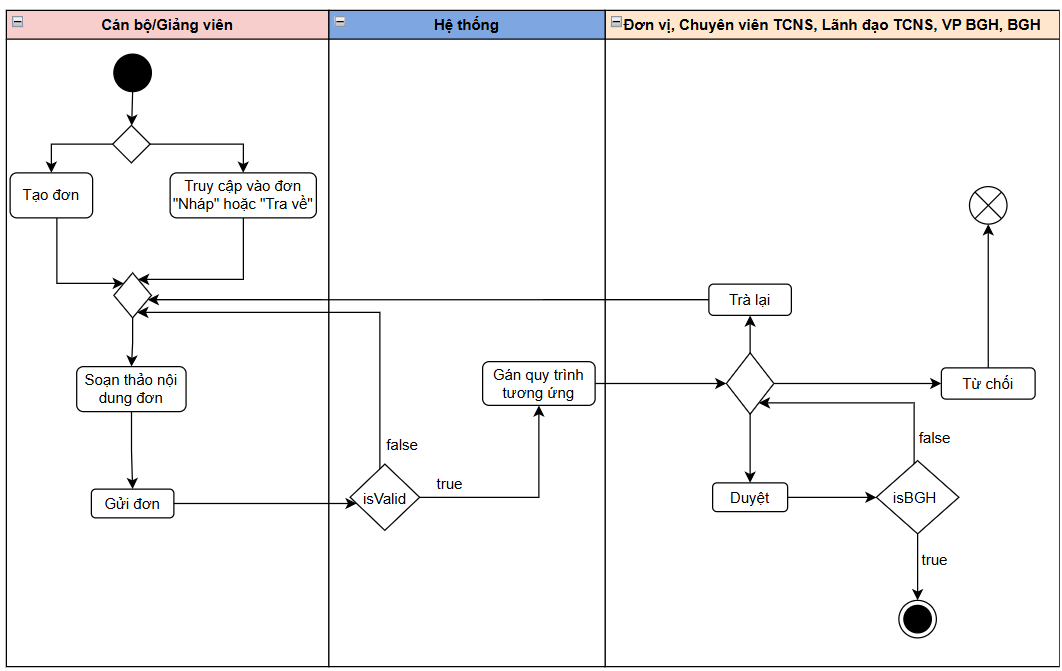
\includegraphics[width=\linewidth]{image/uml/bt_activity.png}
    \caption{\textit{Sơ đồ hoạt động quản lý công tác}}
    \label{fig:BT_AC}
\end{figure}

\subsubsection{Biểu đồ tuần tự}
\begin{figure}[H]
    \centering
    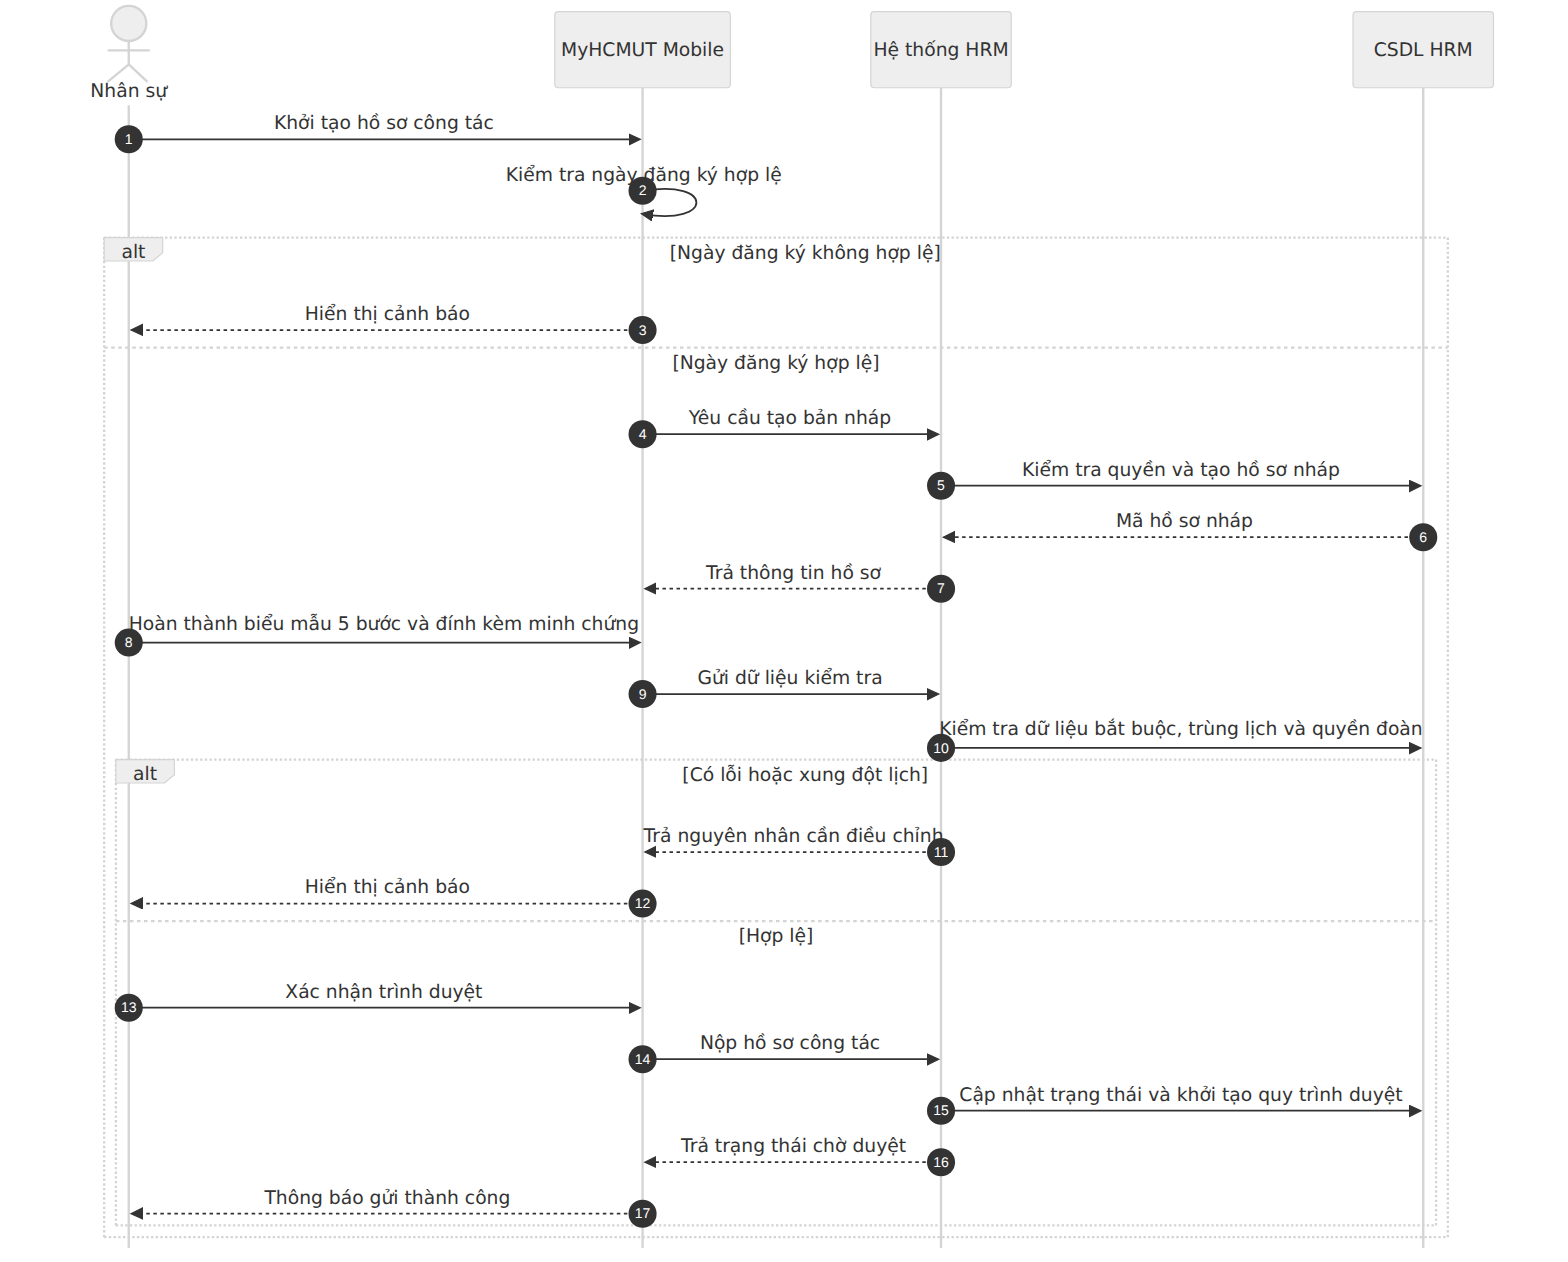
\includegraphics[width=\linewidth]{image/uml/seq_trip_submit.png}
    \caption{\textit{Sơ đồ tuần tự quản lý công tác}}
    \label{fig:BT_SEQ}
\end{figure}

\subsection{Văn phòng số, nhiệm vụ và lịch công tác}
\label{subsec:module_ioffice}
\label{subsec:req_ioffice}
\label{subsec:req_schedule}

\subsubsection{Mục tiêu và yêu cầu chức năng}

Nhóm chức năng Văn phòng số, nhiệm vụ và lịch công tác hỗ trợ cán bộ, giảng viên tiếp cận thông tin điều hành từ hệ thống iOffice trên thiết bị di động: tra cứu văn bản đến/đi, theo dõi thông tin nhiệm vụ được giao và xem lịch làm việc tuần.

Đối với lịch công tác, MyHCMUT Mobile đóng vai trò là cổng hiển thị thống nhất (\textit{Unified Calendar}), tổng hợp các sự kiện có liên quan trực tiếp đến người dùng từ ba nguồn dữ liệu độc lập: lịch họp cơ quan từ iOffice, khoảng thời gian nghỉ phép từ HRM và các chuyến đi công tác từ HRM. Việc tổng hợp này giúp cán bộ có góc nhìn toàn diện về lịch trình cá nhân trên một giao diện duy nhất; trong đó dữ liệu nghiệp vụ gốc vẫn được quản lý và phân định thẩm quyền độc lập tại từng hệ thống nguồn.

Đối với các cuộc họp có yêu cầu điểm danh, ứng dụng hỗ trợ đại biểu ghi nhận trạng thái có mặt hoặc gửi báo vắng có lý do giải trình. Hệ thống máy chủ iOffice đóng vai trò kiểm soát độc lập các điều kiện nghiệp vụ: đại biểu phải có tên trong danh sách mời, cuộc họp đã được kích hoạt tính năng điểm danh và thời điểm thao tác phải nằm trong khung thời gian hợp lệ do ban tổ chức cấu hình.

Bảng~\ref{tab:fr_ioffice_schedule} tổng hợp các yêu cầu chức năng của nhóm nghiệp vụ này.

\begin{table}[H]
\centering
\small
\caption{Yêu cầu chức năng nhóm Văn phòng số, nhiệm vụ và lịch công tác}
\label{tab:fr_ioffice_schedule}
\begin{tabularx}{\textwidth}{|L{1.8cm}|L{3.5cm}|L{2.5cm}|Y|}
\hline
\textbf{Mã FR} & \textbf{Chức năng} & \textbf{Tác nhân} & \textbf{Mô tả và ràng buộc nghiệp vụ} \\
\hline
FR-OFF-01 & Tra cứu văn bản đến và đi & Cán bộ, Giảng viên & Xem danh sách văn bản, tìm kiếm, lọc theo mức độ khẩn và xem tài liệu số đính kèm theo quyền. \\
\hline
FR-OFF-02 & Tra cứu thông tin nhiệm vụ & Cán bộ, Lãnh đạo & Tra cứu danh sách nhiệm vụ được giao hoặc giao đi và xem thông tin được cấp quyền, như trạng thái hoặc hạn xử lý. \\
\hline
FR-SCH-01 & Điểm danh và báo vắng & Cán bộ (Đại biểu) & Ghi nhận có mặt hoặc báo vắng có lý do trong khung thời gian và điều kiện hợp lệ. \\
\hline
FR-SCH-02 & Xem lịch công tác tổng hợp & Cán bộ, Giảng viên & Hiển thị lịch tuần tổng hợp từ 3 nguồn: lịch họp iOffice, lịch phép HRM và lịch công tác HRM. \\
\hline
\end{tabularx}
\end{table}

\subsubsection{Đặc tả Use Case}

Các use case của nhóm chức năng này tập trung vào mục tiêu tra cứu văn bản, theo dõi thông tin nhiệm vụ, xem lịch công tác tổng hợp và thực hiện điểm danh cuộc họp. Hình~\ref{fig:uc_ioffice_schedule} thể hiện sơ đồ use case của nhóm này.

\begin{figure}[H]
\centering
\fbox{\parbox[c][5.5cm][c]{0.85\linewidth}{\centering \textbf{Sơ đồ Đặc tả Use case Văn phòng số, Nhiệm vụ và Lịch công tác} \newline \textit{(Gồm tác nhân Cán bộ/Giảng viên, Đại biểu cuộc họp và các use case UC-OFF-01, UC-SCH-01, UC-SCH-02)}}}
\caption{Sơ đồ Đặc tả Use case nhóm Văn phòng số, nhiệm vụ và lịch công tác}
\label{fig:uc_ioffice_schedule}
\end{figure}

Bảng~\ref{tab:mapping_uc_ioffice} tổng hợp danh mục các use case thuộc nhóm chức năng này.

\begin{table}[H]
\centering
\small
\caption{Danh mục Đặc tả Use case nhóm Văn phòng số, nhiệm vụ và lịch công tác}
\label{tab:mapping_uc_ioffice}
\vspace{0.15cm}
\begin{tabularx}{\textwidth}{|L{2.6cm}|L{4.5cm}|Y|}
\hline
\textbf{Mã Use Case} & \textbf{Tên Use Case} & \textbf{Mục tiêu Nghiệp vụ} \\
\hline
\textbf{UC-OFF-01} & Tra cứu văn bản và nhiệm vụ & Tra cứu văn bản đến/đi, xem tệp đính kèm và theo dõi thông tin các nhiệm vụ được giao trong phạm vi quyền truy cập. \\
\hline
\textbf{UC-SCH-01} & Điểm danh hoặc báo vắng cuộc họp & Ghi nhận có mặt hoặc báo vắng kèm lý do khi tham dự cuộc họp có cấu hình điểm danh. \\
\hline
\textbf{UC-SCH-02} & Xem lịch công tác tổng hợp & Xem các sự kiện từ 3 nguồn dữ liệu (lịch họp iOffice, lịch phép HRM, lịch công tác HRM). \\
\hline
\end{tabularx}
\end{table}

Đặc tả Use casecó nhiều điều kiện nghiệp vụ đáng chú ý là \textbf{UC-SCH-01} được đặc tả chi tiết tại Bảng~\ref{tab:uc_sch_01}. Các use case \textbf{UC-OFF-01} và \textbf{UC-SCH-02} được đặc tả tại Bảng~\ref{tab:uc_off_01} và Bảng~\ref{tab:uc_sch_02}.

\usecasespec{
  id={UC-OFF-01},
  name={Tra cứu văn bản và nhiệm vụ},
  shortname={Tra cứu văn bản \& nhiệm vụ},
  actor={Cán bộ / Giảng viên, Lãnh đạo Đơn vị},
  desc={Cho phép người dùng tra cứu văn bản đến/đi, xem tệp đính kèm và theo dõi thông tin các nhiệm vụ được giao trong phạm vi quyền hạn.},
  pre={Người dùng đã đăng nhập thành công vào ứng dụng MyHCMUT Mobile.},
  trigger={Người dùng chọn mục ``Văn bản'' hoặc ``Nhiệm vụ'' trên ứng dụng.},
  mainflow={
    1. Người dùng mở danh sách văn bản (hoặc nhiệm vụ) trên ứng dụng. \newline
    2. Hệ thống hiển thị danh sách các mục theo quyền truy cập của tài khoản. \newline
    3. Người dùng lọc theo phân loại, trạng thái hoặc tìm kiếm theo từ khóa tiêu đề. \newline
    4. Chọn xem chi tiết một văn bản (hoặc nhiệm vụ) cụ thể để kiểm tra thông tin được cấp quyền.
  },
  altflow={
    - \textit{Luồng 4a (Xem tệp tài liệu số):} Người dùng chọn mở tệp PDF đính kèm để đọc trực tiếp trên ứng dụng.
  },
  exflow={
    - \textit{Ngoại lệ 4a (Không có quyền xem tệp đính kèm):} Hệ thống thông báo văn bản bảo mật và giới hạn quyền truy cập tệp.
  },
  post={Người dùng nắm bắt được thông tin văn bản và nhiệm vụ được cấp quyền truy cập.},
  label={tab:uc_off_01}
}

\usecasespec{
  id={UC-SCH-01},
  name={Điểm danh hoặc báo vắng cuộc họp},
  shortname={Điểm danh cuộc họp},
  actor={Cán bộ / Giảng viên có tên trong danh sách mời},
  desc={Cho phép đại biểu ghi nhận có mặt hoặc báo vắng kèm lý do giải trình đối với cuộc họp có cấu hình điểm danh.},
  pre={Người dùng đã đăng nhập, có tên trong danh sách mời và cuộc họp được cấu hình tính năng điểm danh.},
  trigger={Người dùng mở màn hình chi tiết cuộc họp trên ứng dụng di động.},
  mainflow={
    1. Người dùng mở xem chi tiết cuộc họp trên giao diện Lịch hoặc từ thông báo nhắc việc. \newline
    2. Ứng dụng hiển thị các thao tác điểm danh phù hợp với trạng thái cuộc họp. \newline
    3. Người dùng chọn điểm danh có mặt hoặc báo vắng và nhập lý do khi cần. \newline
    4. Ứng dụng gửi yêu cầu đến iOffice; iOffice kiểm tra tính hợp lệ của đại biểu, cuộc họp và khung thời gian cho phép. \newline
    5. iOffice ghi nhận kết quả và phản hồi trạng thái tham dự mới để ứng dụng cập nhật thông tin hiển thị.
  },
  altflow={
    - \textit{Luồng 3a (Chuyển đổi trạng thái):} Trong khung giờ hợp lệ, người dùng có thể cập nhật lại giữa trạng thái có mặt và báo vắng.
  },
  exflow={
    - \textit{Ngoại lệ 4a (Ngoài khung thời gian):} Thao tác thực hiện ngoài khung giờ quy định $\rightarrow$ hệ thống từ chối và thông báo lý do. \newline
    - \textit{Ngoại lệ 4b (Không thuộc danh sách mời):} Người dùng không có tên trong danh sách đại biểu $\rightarrow$ hệ thống từ chối thao tác.
  },
  post={Trạng thái tham dự được ghi nhận và kết quả mới được phản hồi trên ứng dụng.},
  label={tab:uc_sch_01}
}

\usecasespec{
  id={UC-SCH-02},
  name={Xem lịch công tác tổng hợp},
  shortname={Xem lịch tổng hợp},
  actor={Cán bộ / Giảng viên},
  desc={Cho phép người dùng theo dõi lịch họp iOffice, lịch nghỉ phép HRM và lịch công tác HRM trên một giao diện tuần duy nhất.},
  pre={Người dùng đã đăng nhập và có quyền truy cập dữ liệu nguồn tương ứng.},
  trigger={Người dùng mở màn hình Lịch công tác trên ứng dụng di động.},
  mainflow={
    1. Người dùng mở mục ``Lịch công tác'' trên ứng dụng. \newline
    2. Ứng dụng đồng thời tải các sự kiện lịch mà người dùng được phép xem từ hệ thống iOffice và HRM. \newline
    3. Ứng dụng hiển thị các sự kiện trên giao diện lịch tuần thống nhất, phân biệt rõ nguồn dữ liệu qua màu sắc và nhãn phân loại. \newline
    4. Người dùng chọn một sự kiện cụ thể để xem chi tiết hoặc chuyển đến màn hình nghiệp vụ liên quan.
  },
  altflow={
    - \textit{Luồng 3a (Lọc theo nguồn dữ liệu):} Người dùng có thể bật/tắt hiển thị từng nguồn lịch (chỉ xem lịch họp hoặc chỉ xem lịch phép/công tác).
  },
  exflow={
    - \textit{Ngoại lệ 2a (Không tải được đầy đủ dữ liệu lịch):} Ứng dụng thông báo trạng thái lỗi và cho phép người dùng thực hiện lại thao tác.
  },
  post={Người dùng có góc nhìn lịch trình toàn diện mà không làm thay đổi hay sai lệch dữ liệu nghiệp vụ gốc.},
  label={tab:uc_sch_02}
}

\subsubsection{Biểu đồ hoạt động}

Quy trình điểm danh và báo vắng cuộc họp có nhiều điều kiện nghiệp vụ liên quan đến người tham dự, trạng thái cuộc họp và thời gian thực hiện, do đó được lựa chọn để mô tả bằng biểu đồ hoạt động.

Hình~\ref{fig:act_attendance} mô tả quy trình điểm danh và báo vắng cuộc họp của UC-SCH-01. Quy trình bắt đầu khi người dùng truy cập một cuộc họp có hỗ trợ điểm danh. Hệ thống kiểm tra các điều kiện thực hiện trước khi cho phép người dùng ghi nhận có mặt hoặc báo vắng kèm lý do. Khi thao tác hợp lệ, trạng thái tham dự được ghi nhận và kết quả được phản hồi trên ứng dụng; trường hợp không đáp ứng điều kiện, hệ thống từ chối thao tác và thông báo nguyên nhân cho người dùng.

\begin{figure}[H]
\centering
\fbox{\parbox[c][7cm][c]{0.85\linewidth}{\centering \textbf{Vị trí biểu đồ hoạt động} \\ \textit{Điểm danh và báo vắng cuộc họp}}}
\caption{Biểu đồ hoạt động Điểm danh và báo vắng cuộc họp}
\label{fig:act_attendance}
\end{figure}

\subsubsection{Biểu đồ tuần tự}

Biểu đồ tuần tự mô tả sự tương tác ở mức logic giữa người dùng, MyHCMUT Mobile và hệ thống iOffice trong quá trình điểm danh hoặc báo vắng cuộc họp. Khi người dùng thực hiện thao tác trên ứng dụng, yêu cầu được chuyển đến hệ thống iOffice để kiểm tra các điều kiện nghiệp vụ và ghi nhận kết quả. Trạng thái tham dự sau xử lý được trả về MyHCMUT Mobile để cập nhật thông tin hiển thị cho người dùng.

Hình~\ref{fig:seq_attendance} thể hiện trình tự tương tác của use case UC-SCH-01. Biểu đồ chỉ tập trung vào sự phối hợp giữa các thành phần ở mức hệ thống; các thành phần hiện thực và cơ chế giao tiếp chi tiết được trình bày tại Chương~5.

\begin{figure}[H]
\centering
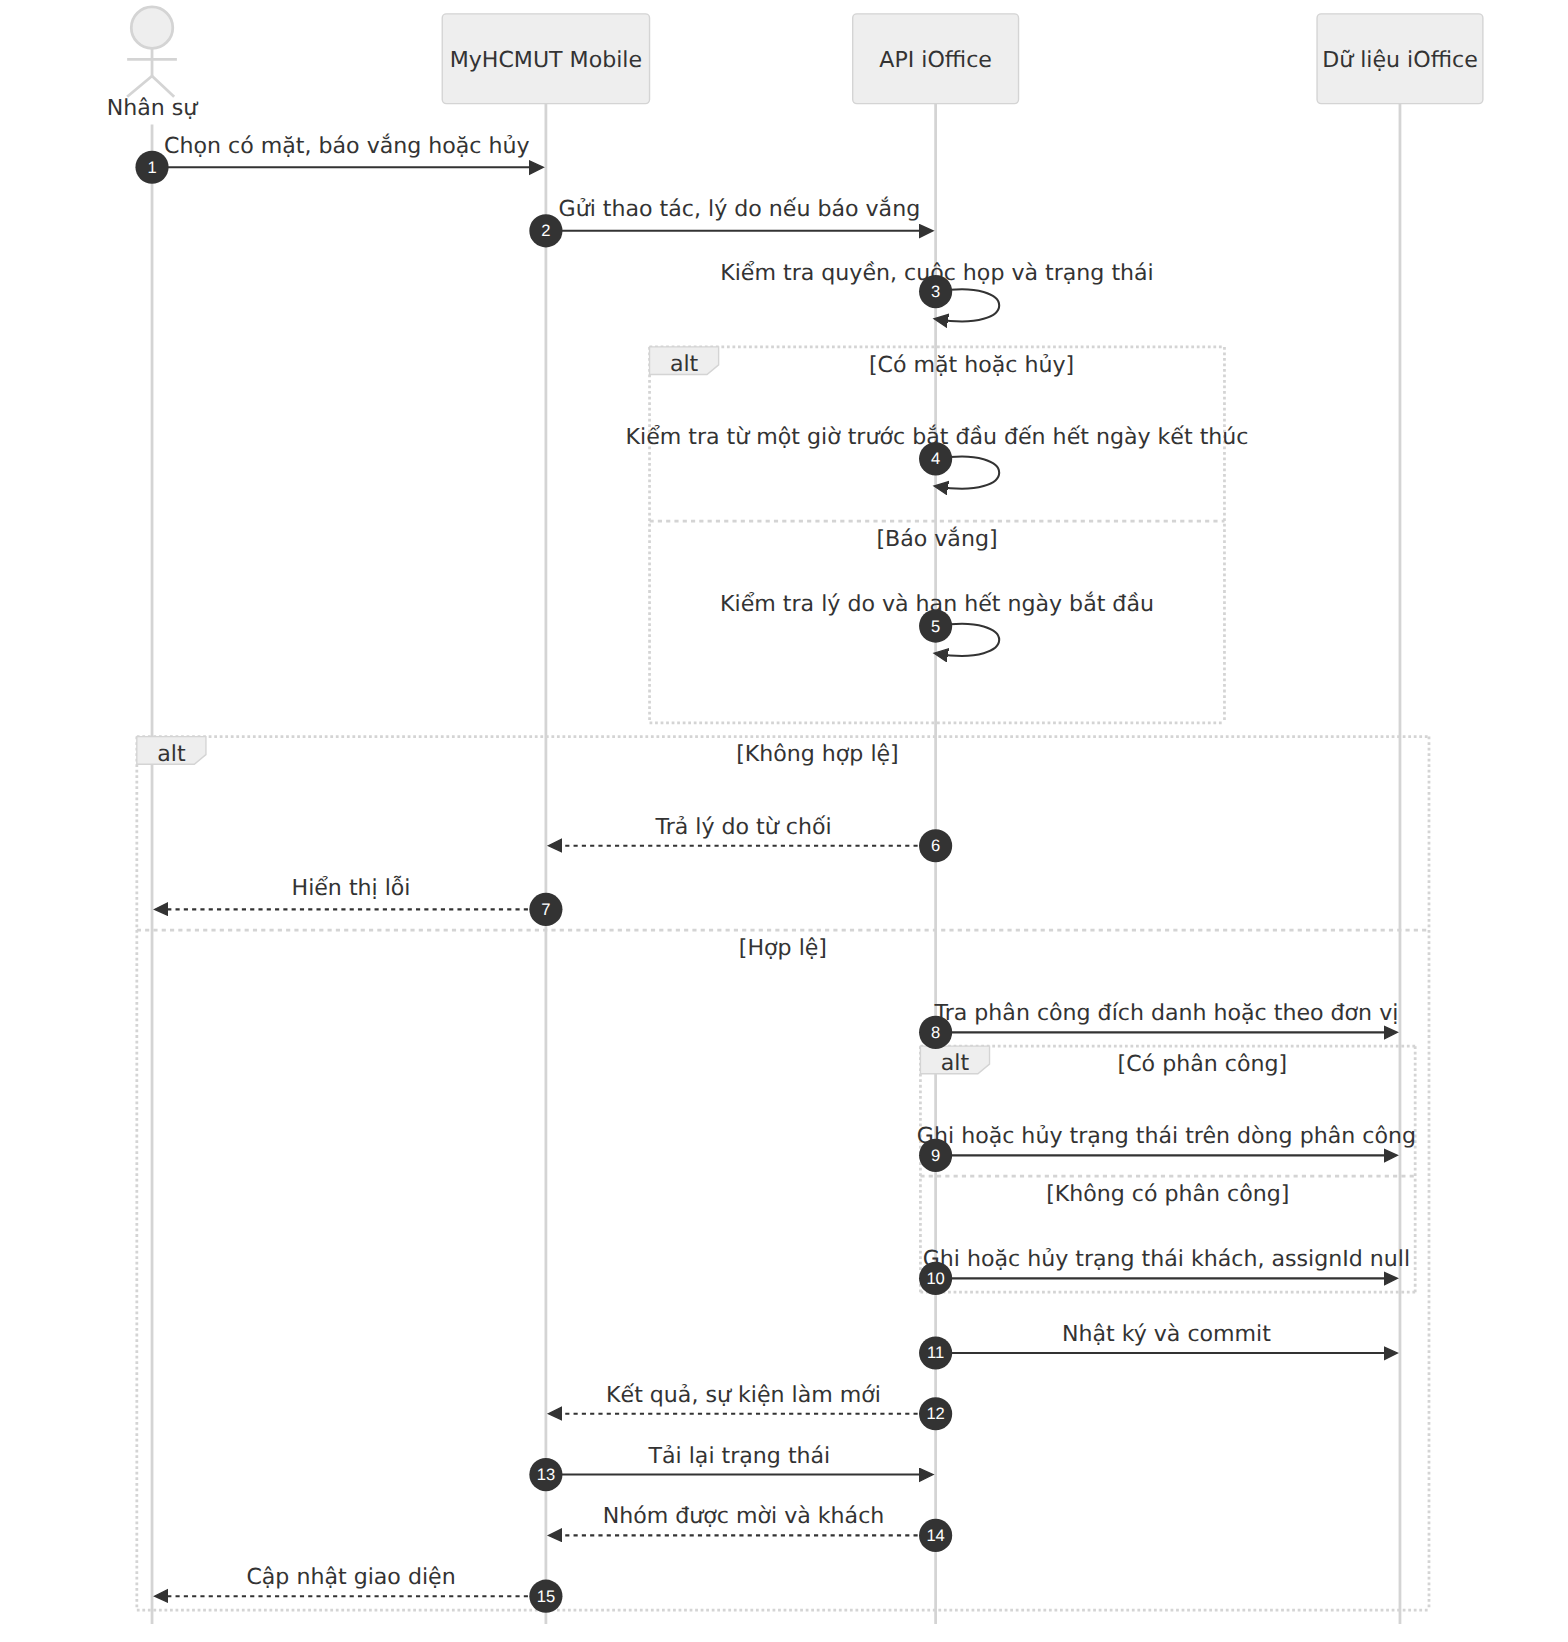
\includegraphics[width=\linewidth]{image/uml/seq_attendance.png}
\caption{Biểu đồ tuần tự Điểm danh và báo vắng cuộc họp}
\label{fig:seq_attendance}
\end{figure}

